\chapter{Introduction}
\label{chap:intro} %este label será usado para referenciar este capítulo

Electrohydrodynamic Atomization (EHDA) is a way to disintegrate a liquid into droplets by exposing it to a strong electric field.\cite{prunet}
The balance beetween capilary forces and the eletric field on the charged liquid defines the spraying dynamics and droplet size.
The electric current transported by the spray reveals characteristic shapes for different spray modes.
Signal processing techniques can allow a non-visual classification of the spray mode based on the electric current shape.\cite{Sjaaks}
The spray process imposes noise and random sequences on the measured signal making its classification not a trivial task. 
Industrial applications demand automated stabilization of a spray mode. 
This can be achieved by a closed-loop control system. 
This project is about to develop an application that can classify what dynamics the EHDA experiment is current in and control the variables to stabilize in the desired mode. 

\section{Droplet Formation}
\label{sec:drop_formation}

In the Aerosol reasearch community there is a branch of studies about droplets formation. In the droplet field a very functional for applications is the atomization, which refers to breaking the liquid in small droplets.
There is many ways of atomizing a liquid. Some using mechanical energy such as ultrassound, rotating disk\cite{Disk_atomization}, pressure or blowing air on the meniscus. But also, some of them using electric forces such as electrospray atomization.

For 


\section{EHDA}
\label{sec:ehda_resume}

The electrospraying of liquids herein is referred to as electrohydrodynamic atomization (EHDA). The atomization by primarily electrical (electro) forces of a liquid (hydro) that is moving (dynamic) during the atomization captures the essence of the phenomena.\cite{Grace}
That motion applies to the liquid certain velocity that is not enough to create the spray alone. Therefore, the eletric field itself is the responsible for the spraying dynamics.\cite{prunet}

The stable balance between the capilary and field forces on the liquid suggest a \emph{quasi static} dynamics.
For this reason with a controlled enviroment we can reach a certain stable spraying mode as can be seen in the Figure \ref{fig:ehda_setup_ex2}.

\begin{figure}[H]
  \centering
  \resizebox{80mm}{!}{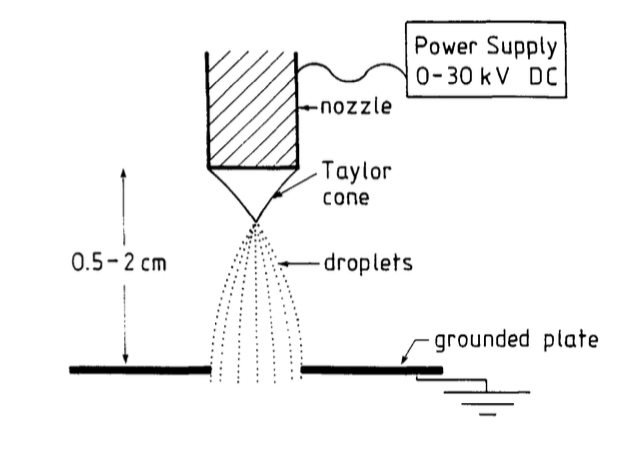
\includegraphics{Figuras/ehda_ex_2.png}}
  \caption{EHDA physical concept \cite{Gabriel}}
  \label{fig:ehda_setup_ex2}
\end{figure}

\section{Spraying modes}
\label{sec:spraying_modes_subsec}

Since 1915 with his pioneering work in EHDA, Zeleny observed several functioning modes with very different characteristics.
Years later the same phenomena was noticed by other scientists but the classification of these modes were still not well defined by the community.
For that Cloupeau and Prunet-Foch proposed spray mode classifications based in what they have seen experimentally and it's still being used as basis for EHDA researchs.\cite{prunet}

The Figures \ref{fig:dripping_camera_example}, \ref{fig:cone_camera_jet_example}, \ref{fig:multi_camera_jet_example} shows the 3 spraying dynamics that we are most intersted in this project. 

\begin{multicols}{3}

  \begin{figure}[H]
      \center
      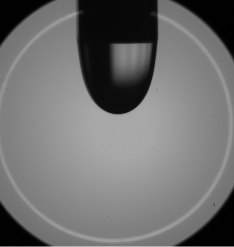
\includegraphics[width=3cm]{Figuras/drippingexample.png}
      \label{fig:dripping_camera_example}
      \caption{Dripping}
  \end{figure}


  \begin{figure}[H]
      \center
      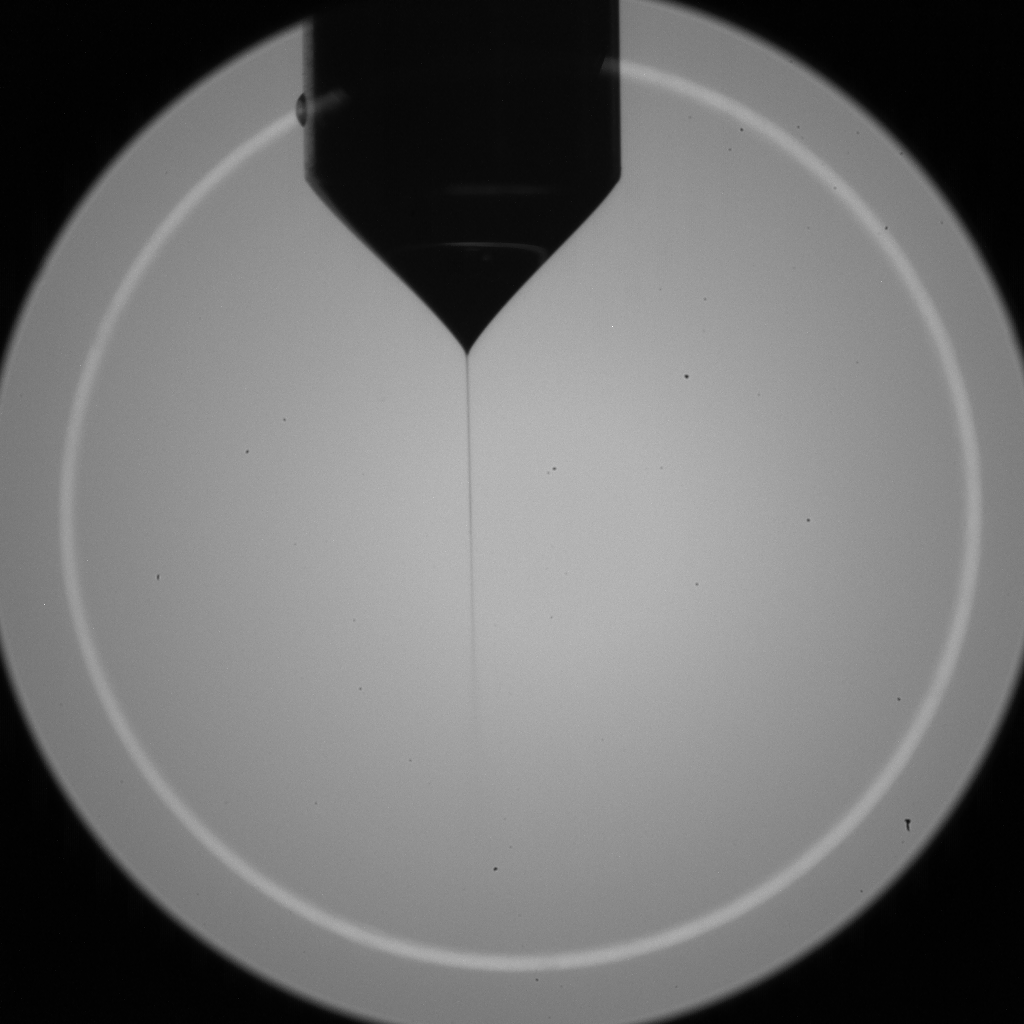
\includegraphics[width=3cm]{Figuras/conejetexample.png}
      \label{fig:cone_camera_jet_example}
      \caption{Cone Jet}
  \end{figure}


  \begin{figure}[H]
      \center
      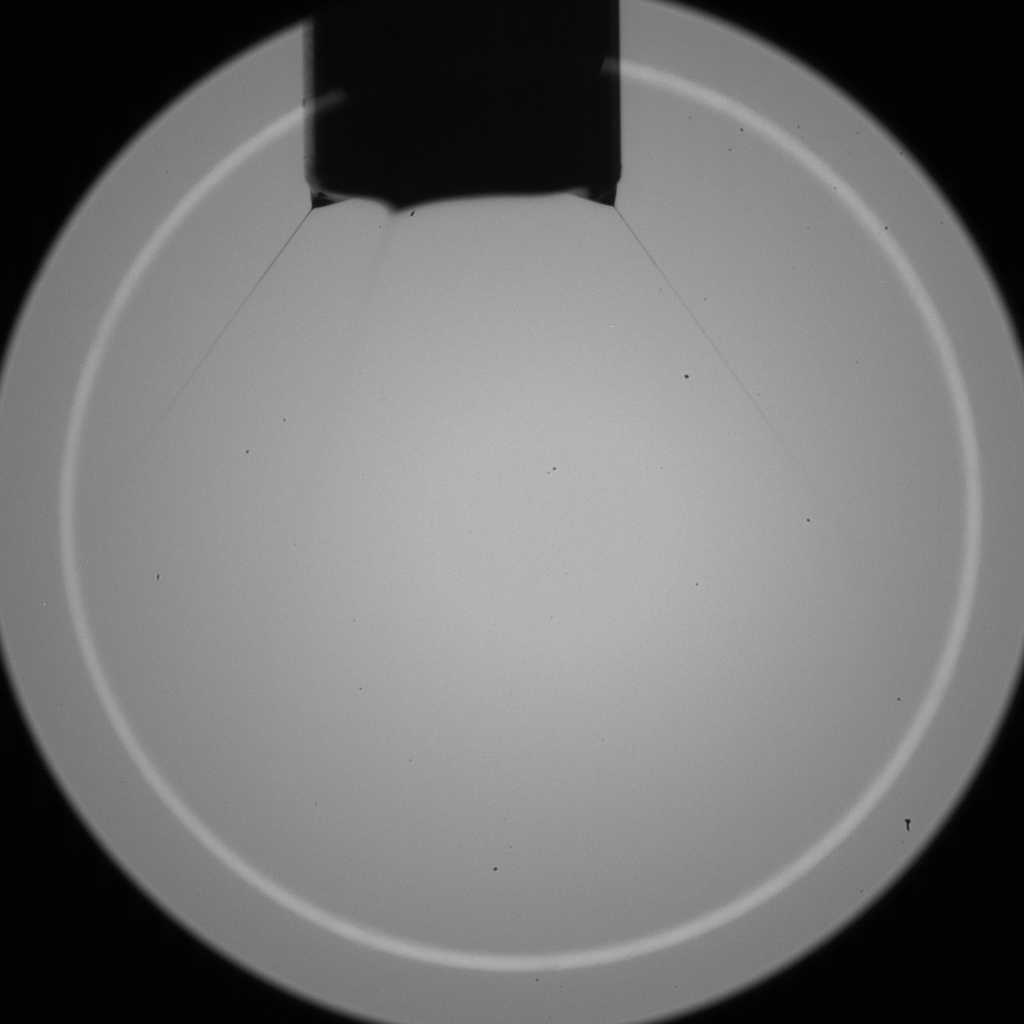
\includegraphics[width=3cm]{Figuras/multijetexample.png}
      \label{fig:multi_camera_jet_example}
      \caption{Multi Jet}
  \end{figure}

\end{multicols}

Through the various classifications defined we are going to work aggregating some of them and separating beetween 5 modes as shown above:

\subsection{Dripping}
\label{subsec:dripping}

In Dripping mode the eletric field applied is not enough to change the meniscus shape, phenomena called field enhanced dripping.
In that situation the liquid droplet has, in general, size bigger than the capilary and low frequency intervals between each drop.

\subsection{Intermittent}
\label{subsec:Intermittent}

Intermittent mode is defined when the eletric field forces starts to have a considerable effect in the meniscus and droplet formation. 
In this mode the droplet size is smaller than the nozzle, phenomena called microdripping, and the dripping frequency increases with the increasing of the field applied.

\subsection{Cone Jet}
\label{subsec:Cone Jet}

\subsection{Multi Jet}
\label{subsec:Multi Jet}

\subsection{Corona sparks}
\label{subsec:Corona sparks}


\section{Non-visual classification}
\label{sec:non-visual-classification}

Since the beginning of EHDA until today the researchs are being conducted manually with visual classification of the spraying mode using a camera or even by naked eyes.
It is recommended to use a high speed (HS) camera because some dripping or intermittent states can be in a high frequency and be wrongly noticed as a stable condition.
The setup in \ref{fig:ehda_setup} shows the most common setup used for EHDA researchers.

\begin{figure}[H]
  \centering
  \resizebox{150mm}{!}{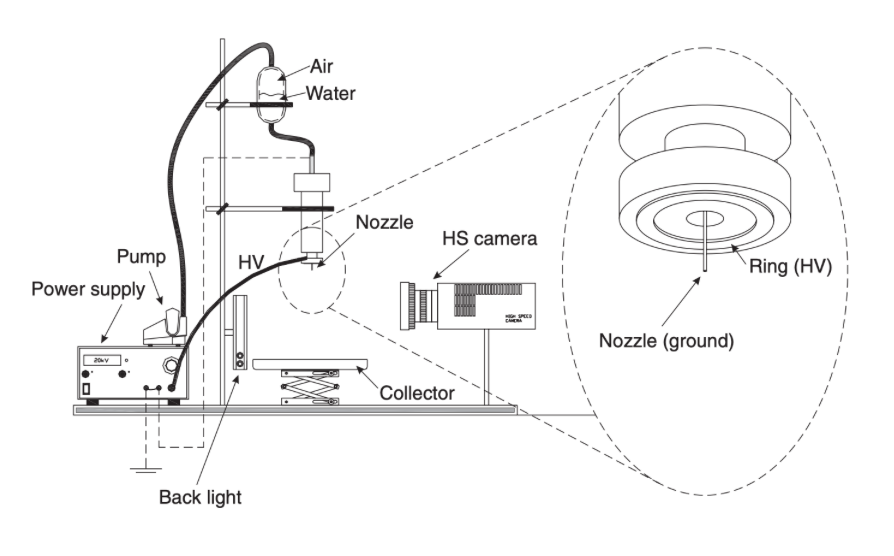
\includegraphics{Figuras/system_setup.png}}
  \caption{EHDA experiment setup \cite{Luewton}}
  \label{fig:ehda_setup}
\end{figure}


Therefore some researchs were made about the classification of the spraying mode measuring the current flowing through the nozzle to plate\cite{Sjaaks}\cite{Chen_Pui}. That current signal holds a lot o information 
about the dynamics that is happening with the liquid. In \ref{fig:microdripping_current_pic} we can see an example of that. It's clear the two droplets generated in this time frame.


\begin{figure}[H]
    \centering
    \resizebox{150mm}{!}{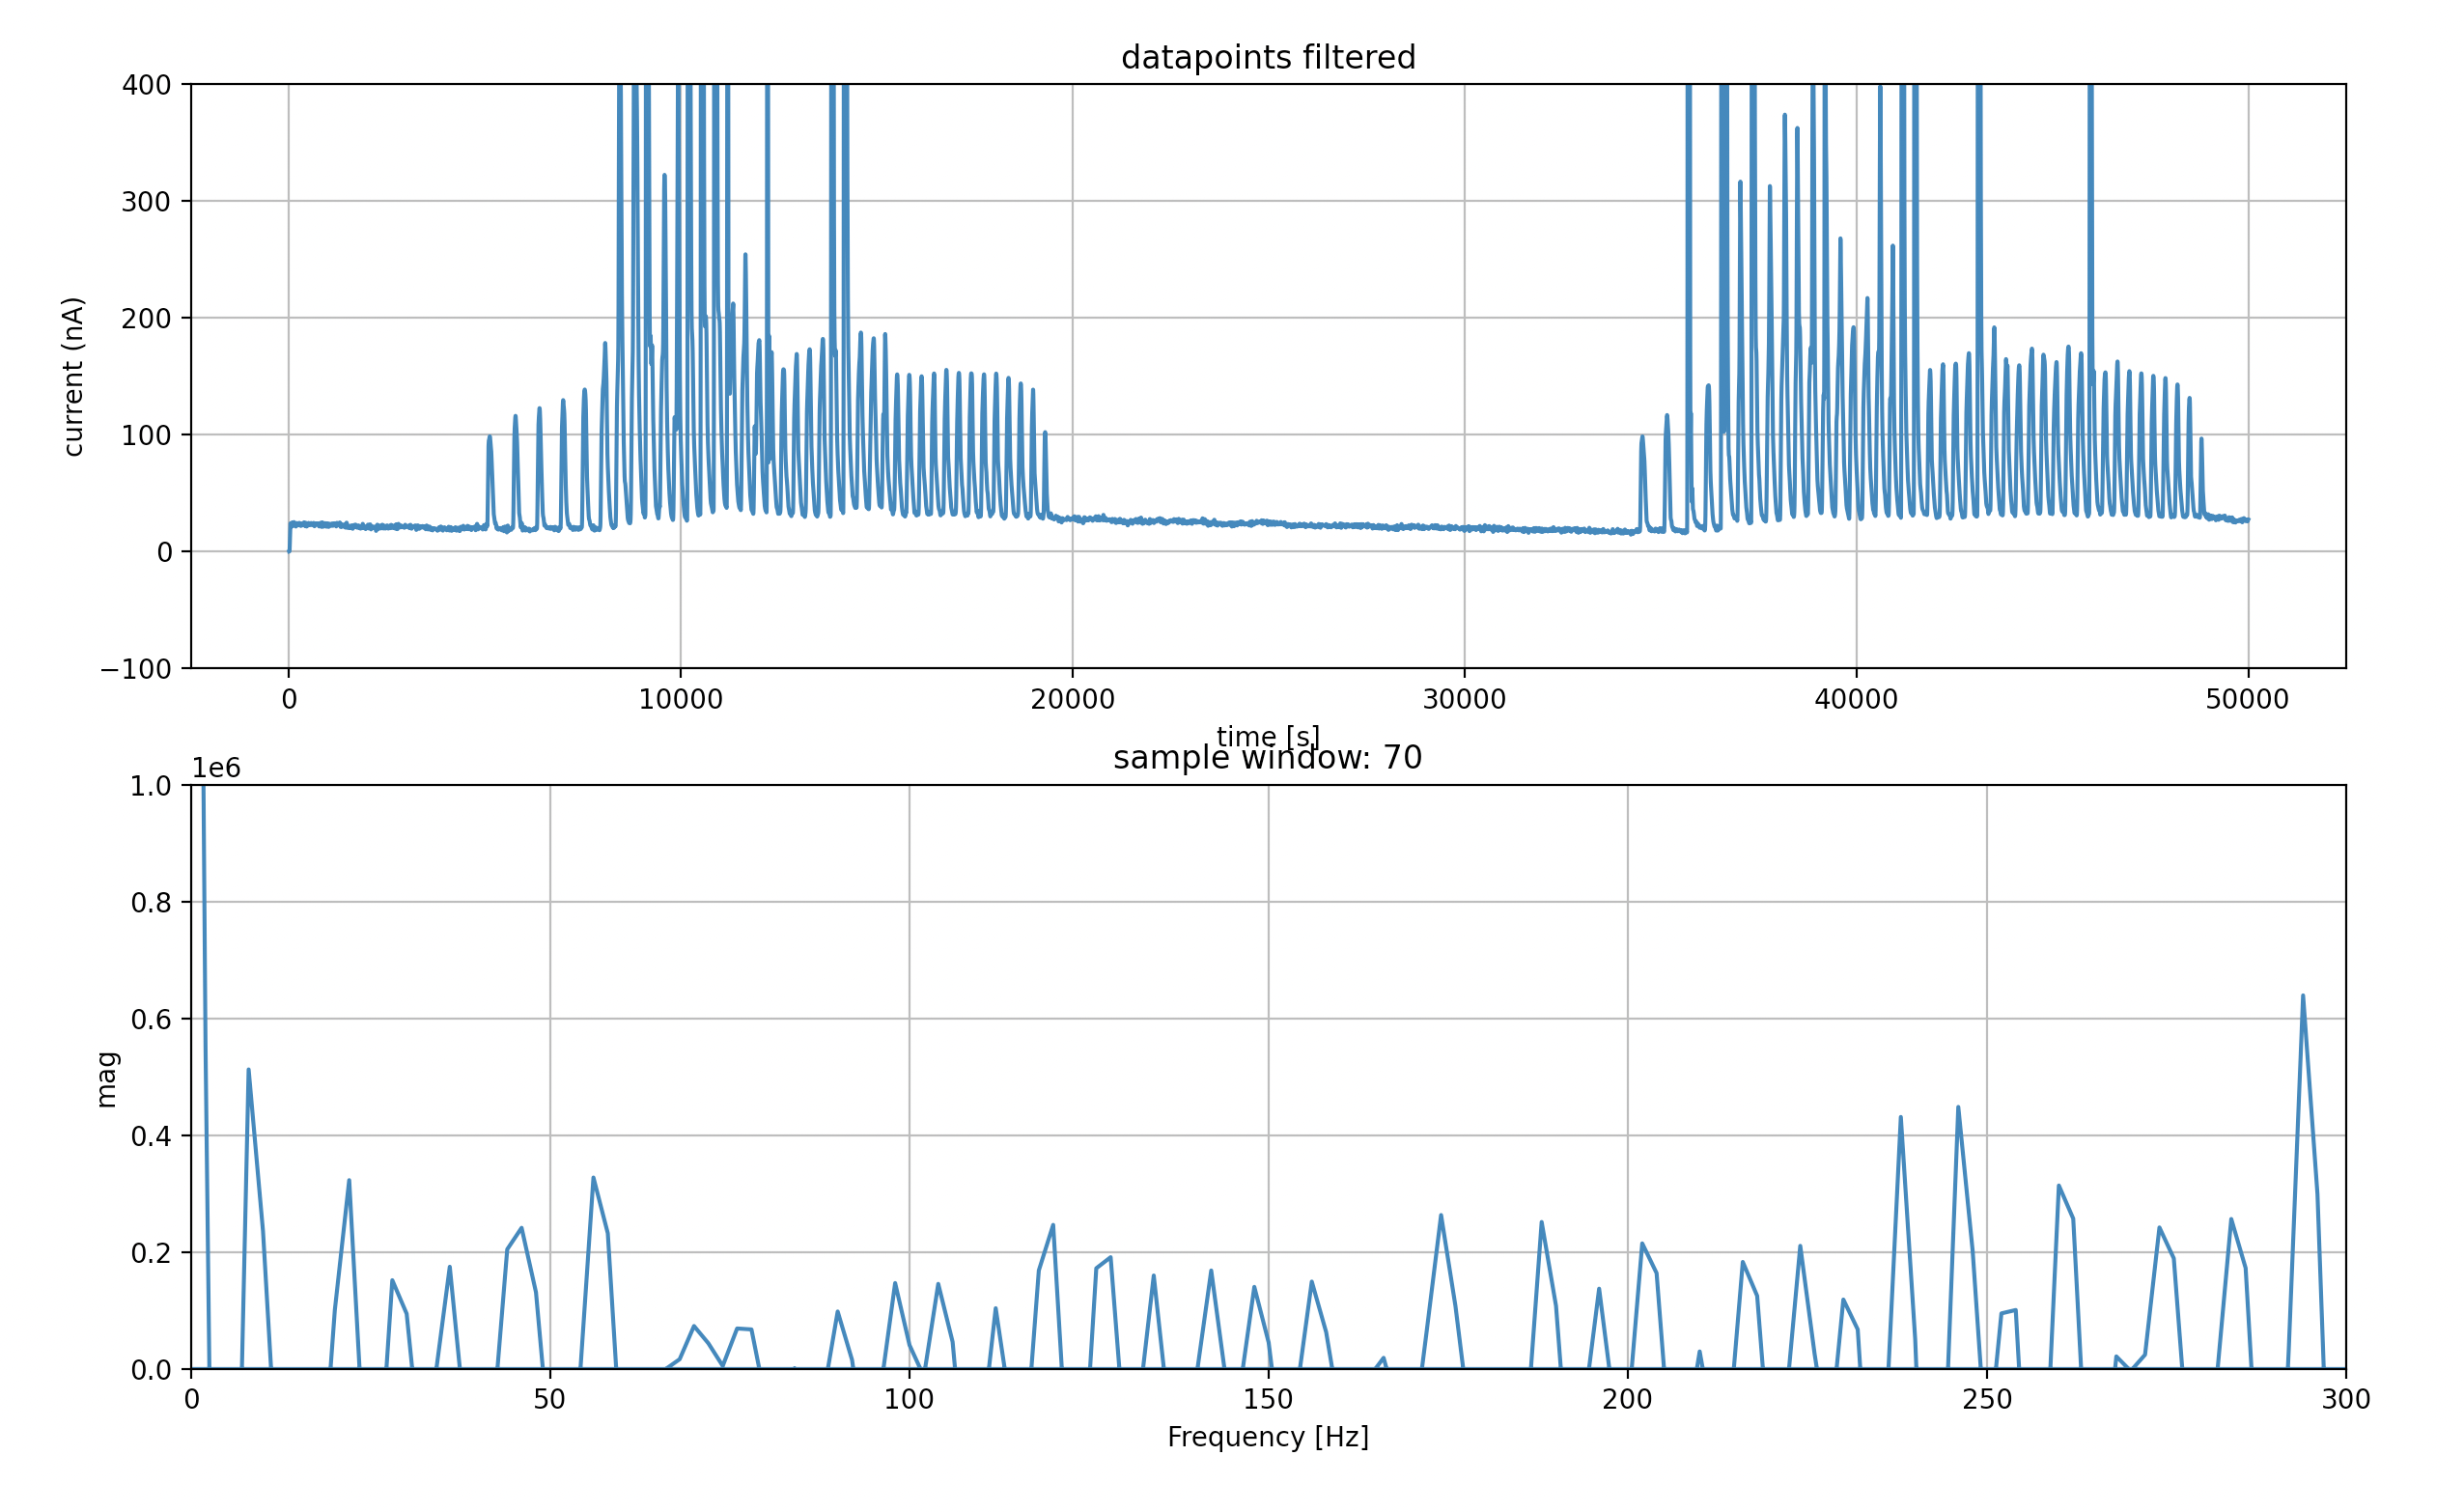
\includegraphics{Figuras/report2/img2.png}}
    \caption{Current measurement sample of a micro-dripping spraying mode. This graph represents 0.5s sample. The sampling frequency is 100kHz. Hence we have 50000 current values.}
    \label{fig:microdripping_current_pic}
  \end{figure}

\section{Motivation and Justify}
\label{sec:motivacao}
% Argumente sobre a importância do projeto desenvolvido usando uma visão de alto nível, sem entrar em detalhes. Contextualize seu projeto dentro do local de execução ou da literatura e explique como ele é necessário ou inovador. É possível fazer uma breve revisão bibliográfica, confrontando seu trabalho com outras referências bibliográficas para mostrar a sua contribuição. No quesito contribuição, é muito importante deixar claro o tempo todo que partes do projetos foram executadas por outros e que partes foram executadas por você. Caso contrário, corre-se o risco de inadvertidademente tomar crédito pelo trabalho de outrem, o que pode ter implicações legais. 

As pesquisas de EHDA têm contribuído como uma importante ferramenta para
o desenvolvimento da tecnologia . Embora existam aplicações de EHDA em
indústria, a estabilização do modo de pulverização de jato cônico é feita empiricamente e com base em medições de corrente média.
A corrente elétrica que flui transportada pelo spray revela formas características para diferentes modos de atomização.
Essas formas não podem ser simplesmente resumidas por seu valor médio. Na figura um podemos ver um exemplo de cone-jet
modo eletrospray.

Figura 1: exemplo de EHDA

As técnicas de processamento de sinal podem permitir uma classificação não visual do modo de pulverização com base no elétrico
forma atual. O processo de pulverização impõe ruídos e sequências aleatórias no sinal medido tornando-o
classificação não é uma tarefa trivial.
Aplicações industriais exigem estabilização automatizada de um modo de pulverização. Isso pode ser obtido por um sistema fechado
sistema de controle de circuito. A classificação automatizada do modo de pulverização é uma parte crucial de um sistema de controle, assim como
o desenvolvimento de um algoritmo de controle apropriado.

\section{Project objectives}
\label{sec:objetivos}

Tendo em vista o exposto acima, este projeto tem por objetivos:

\begin{enumerate}[a)]
\item Item 1;
\item Item 2; 
\item Etc.     
\end{enumerate}

O conteúdo desta seção pode se sobrepor um pouco com o da seção anterior, podendo ela ser um sumário dos pontos expostos anteriormente. A escolha do título da seção talvez seja mais apropriada para a fase de proposta do projeto. Afinal, nesta fase se conhecem os objetivos e não os resultados. Por outro lado, fará pouco sentido discutir objetivos quando o projeto está finalizado, especialmente se tais objetivos não foram alcançados. 


\section{People envolved}
\label{sec:empresa}

% Faça uma breve apresentação da empresa ou laboratório onde o projeto é desenvolvido. Fale um pouco da história da empresa, do mercado em que atua, da sua organização, do departamento em que está inserido o projeto, etc. Descreva também o seu vínculo com a empresa. 
Implementações de processamento de sinal de projetos anteriores
do grupo NHL Stenden Water Technology estão mostrando bons resultados de classificação. Mais pesquisas são
necessário para melhorar a precisão da classificação e pesquisa e implementação de uma classificação adequada
algoritmo. Por causa disso, o trabalho será feito pelo Water Technology Group da NHL Stenden University
de Ciências Aplicadas e em combinação com empresas holandesas para combinar possibilidades de análise com conhecimento
e disponibilidade de infraestrutura.


\clearpage